\section{Simulation}

In order to test our approach composed a path using 8 markers and made the quadrotor follow it. The path is shown in Figure \ref{fig:path} where each marker is a square of 20cm side and the distance between each of them is 50cm; the quadrotor follows the path at a constant height of 2m. The size, the number and the distances of the tags, as well as the height of the quadrotor and the shape of the path, can be arbitrarily changed; the only restriction is that at least one tag need to be in the field of vision of the robot for all the duration of the simulation.

\begin{figure}[h!]
  \centering
    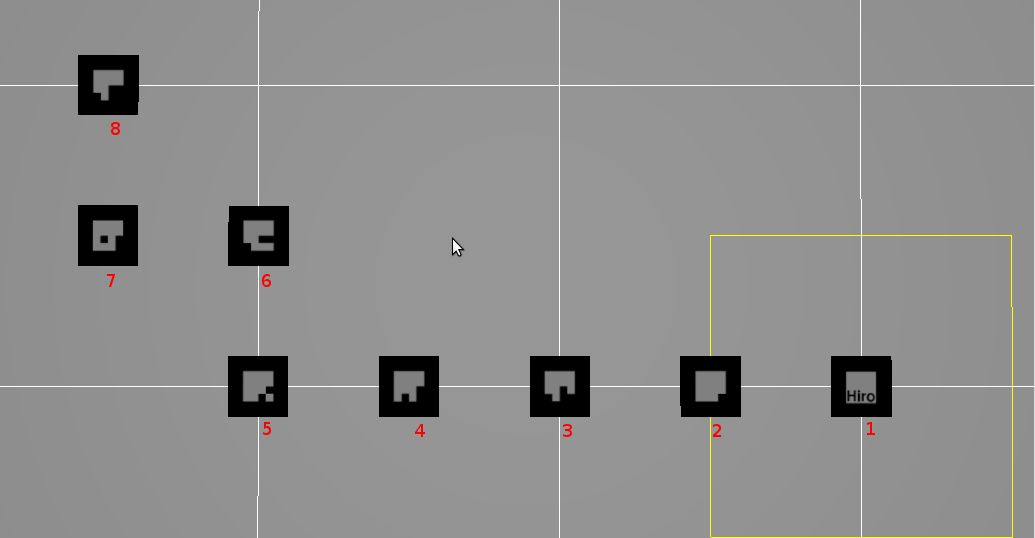
\includegraphics[scale=0.35]{figs/path.png}
  \caption{The path followed by the quadrotor during the simulations}
  \label{fig:path}
\end{figure}


In Figure \ref{fig:plot} we show the result of the first simulation. It can be seen that the estimate position along $X$ and $Y$ is very close to the real one, measured directly form the simulated environment. The plot for the position along the $Z$ axis appears at first more noisy but at a closer inspection we notice that the variation are in the order of $\pm$ 0.03 m that is very close to the maximum accuracy of ARTag ($\pm$ 0.02m).

\begin{figure}[h!]
  \centering
    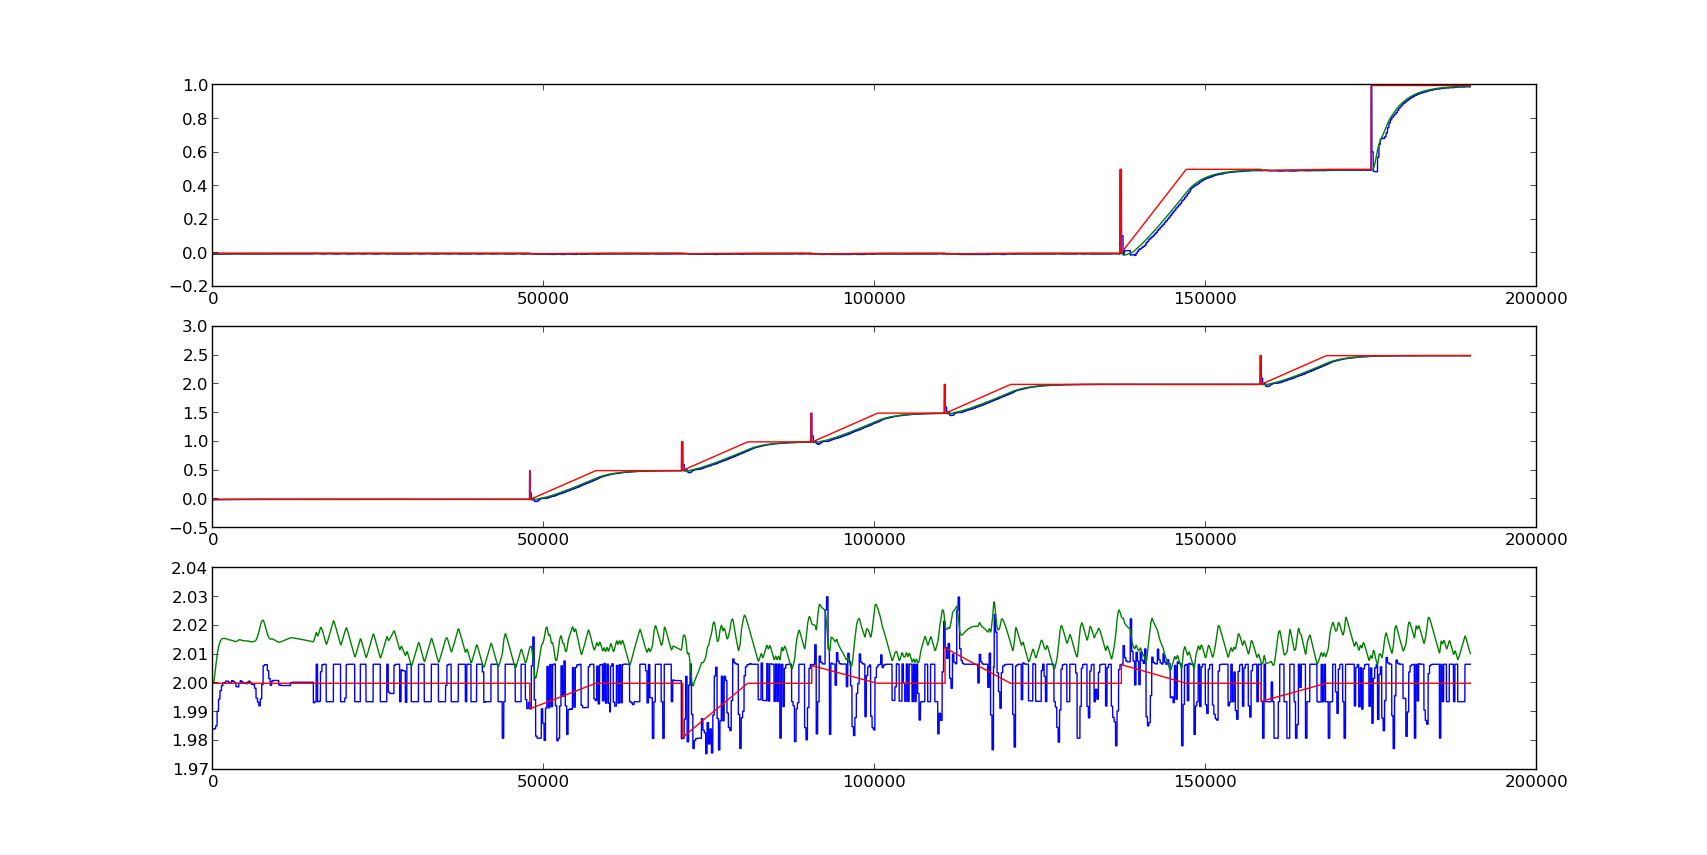
\includegraphics[scale=0.35]{figs/plot.png}
  \caption{Plot of desired, estimated and actual values for the position of the quadrotor}
  \label{fig:plot}
\end{figure}


To test the robustness of our approach and to better model real-environment conditions we ran a second simulation where we artificially introduced some disturbances. These disturbances were implemented in two different ways, first we added both a Gaussian and a RGB noise on the image of the camera, Figure \ref{fig:artag} shows the difference of the perceived marker before and after the noise was added.

 \begin{figure}[!h]
 \centering
 \subfigure[ARTag with no noise]
   {
\includegraphics[width=4cm]{figs/artag.png}}
 \hspace{5mm}
 \subfigure[ARTag with Gaussian and RGB noise]
   {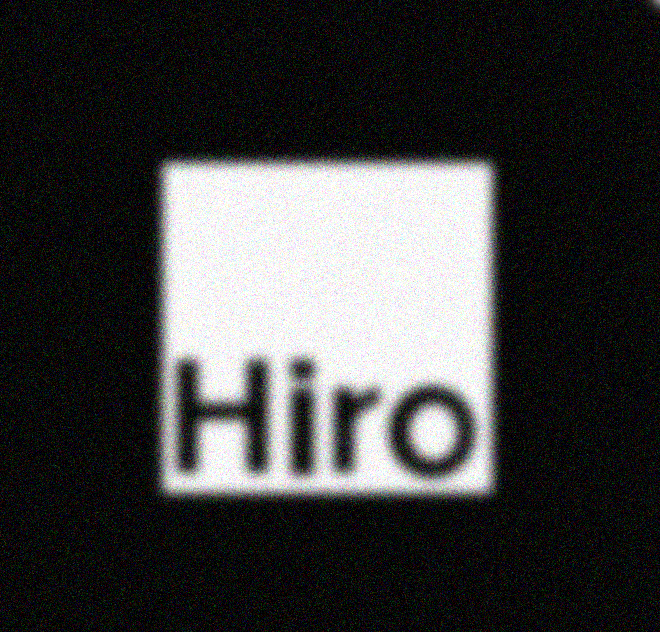
\includegraphics[width=4cm]{figs/artag_noise.png}}
 \caption{Difference between tag wit and without noise}
 \label{fig:artag}
 \end{figure}
 

The second type of disturbance was introduced directly on the estimate of the position of ARTag by adding a Gaussian noise to it. To do so we computed a Gaussian distribution with $\mu=0$ and $\sigma^2=1$, according to the Box-Muller algorithm, scaled it by a constant factor $k=0.05$ and then we added it to the estimate by ARTag. In Figure \ref{fig:plot_noise} we show the result of this second simulation.

\begin{figure}[h!]
  \centering
    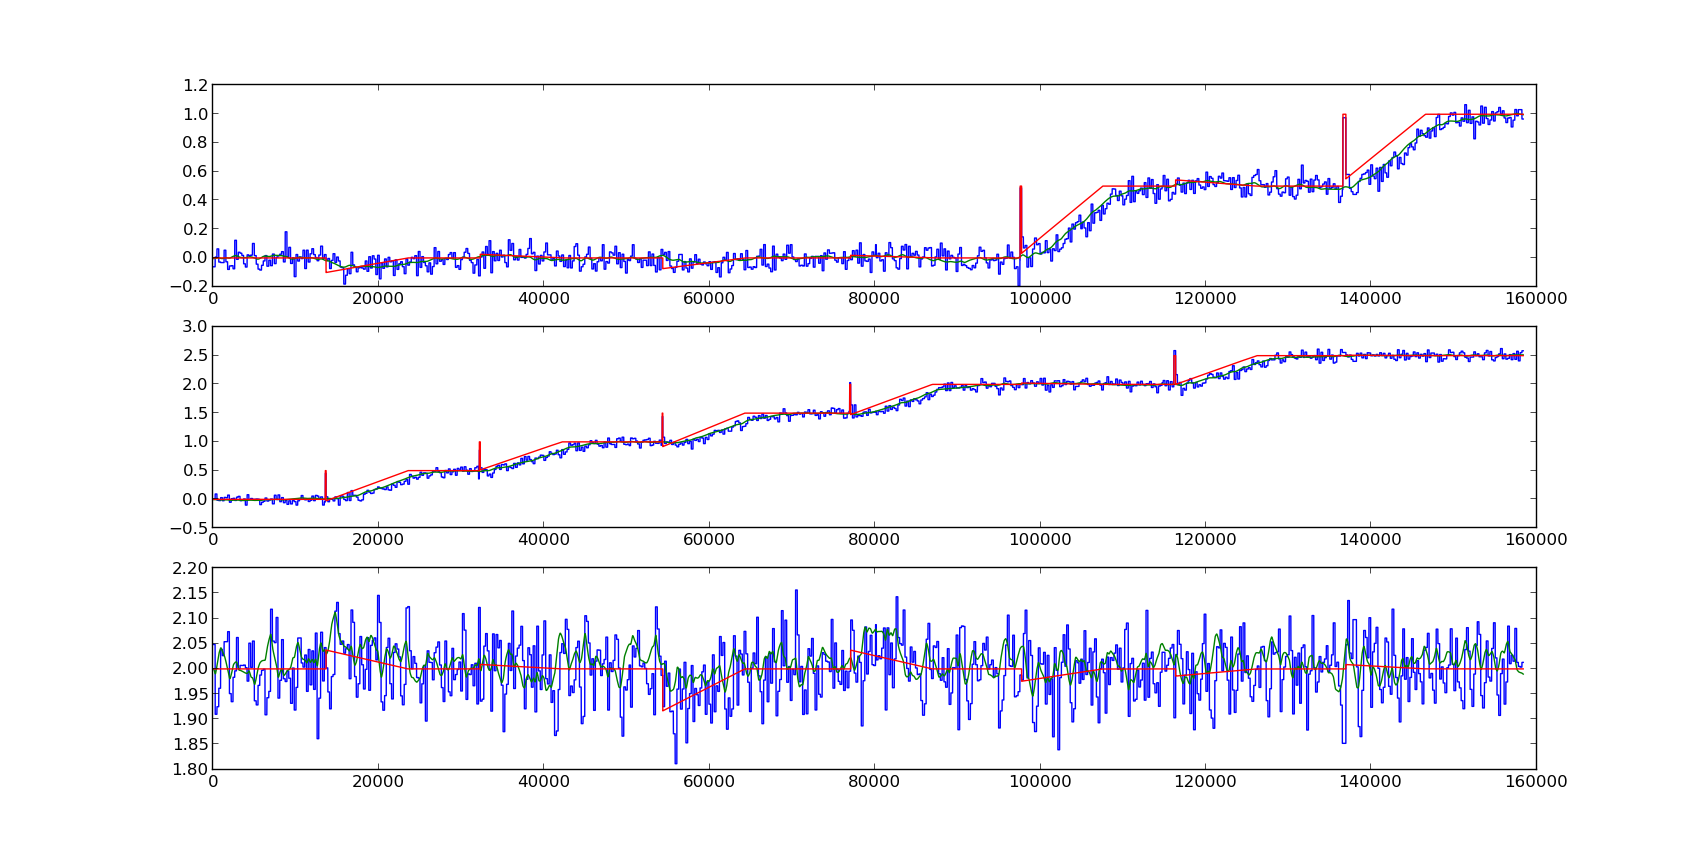
\includegraphics[scale=0.35]{figs/plot_noise.png}
  \caption{Plot of desired, estimated and actual values for the position of the quadrotor when noise was added}
  \label{fig:plot_noise}
\end{figure}


As can be seen even though some strong disturbance was introduced the estimate position is still close to the real one and the quadrotor is able to follow the path as planned. For this reason we believe that our approach could be applied not only in a simulation but to a real robot as well.